\begin{frame}{Pre-installazione}
    Prima di procedere con l'installazione dobbiamo "architettare"
    il nostro sistema.
    \begin{itemize}
        \item \textbf{Disco}
        \begin{enumerate}
            \item Partizionamento
            \item Filesystem
            \item Cifratura
        \end{enumerate}
        \item \textbf{Display Server}
        \item \textbf{Desktop Environment}
        \item ...
    \end{itemize}
\end{frame}
%------------------------------------------------
\begin{frame}{Disco(1) - Partizionamento}
Per questa installazione faremo un partizionamento abbastanza semplice:
\vspace{20pt}
\begin{center}
    \begin{tabular}{ | m{7em} | m{8em} | m{5em}| m{5em} | } 
        \hline
        \textbf{Tipo partizione} & \textbf{Punto di mount} & \textbf{Filesystem} & \textbf{Dimensione} \\ 
        \hline
        Boot/EFI & /boot & FAT32 & 500MB \\ 
        \hline
        Root & / & BTRFS & 31.5GB \\ 
        \hline
        Swap & /swap & - & 8GB \\
        \hline
    \end{tabular}
\end{center}
\vspace{20pt}
Per la dimensioni delle partizioni si presuppone di avere un disco di 40GB.
\end{frame}

%------------------------------------------------

\begin{frame}{Perché BTRFS?}

\end{frame}

%------------------------------------------------

\begin{frame}{Disco(3) - Cifratura}
    \begin{figure}[h]
        
\includegraphics[width=0.3\textwidth]{images/encryption.png}
    \end{figure}
I sistemi GNU/Linux supportano 2 tipi di cifratura del disco:
\begin{itemize}
    \item Cifratura stacked system (eCryptfs, EncFS)
    \item Cifratura dei dispositivi a blocchi: dm-crypt+LUKS
\end{itemize}
\end{frame}

%------------------------------------------------

\begin{frame}{Cifratura stacked system: eCryptfs}
    \begin{figure}[h]
        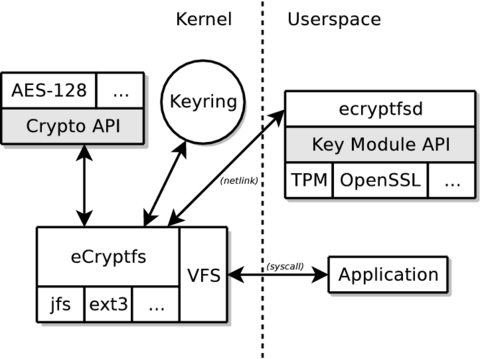
\includegraphics[width=0.4\textwidth]{images/ecryptfs.jpg}
    \end{figure}
\begin{itemize}
    \item Cifratura on-the-fly
    \item Utilizzo di uno "strato cuscinetto" per cifrare/decifrare i dati
    \item Possibilità di cifrare dischi "a caldo"
    \item Non cifra i metadati
\end{itemize}
\end{frame}

%------------------------------------------------

\begin{frame}{Cifratura a blocchi: dm-crypt+LUKS}
    \begin{figure}[h]
        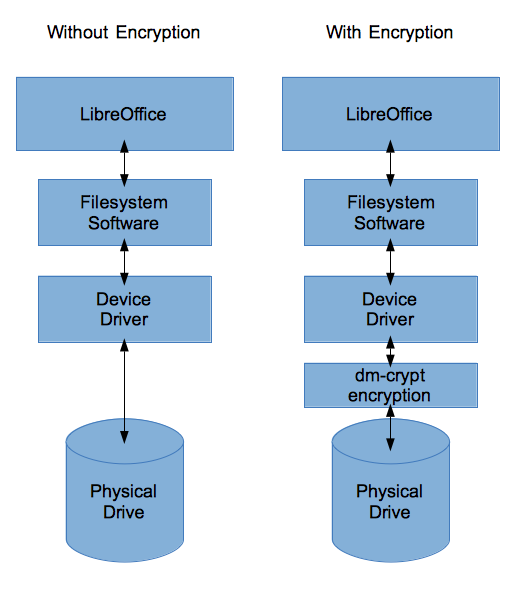
\includegraphics[width=0.4\textwidth]{images/dm-crypt.png}
    \end{figure}
\begin{itemize}
    \item Opera al di sotto del filesystem
    \item Cifratura solo a "freddo"
    \item Più veloce (anche se parliamo di casi d'uso differenti)
\end{itemize}
\end{frame}

%------------------------------------------------
\begin{frame}{Display Server}
    %Il \textbf{display server} è la componente software responsabile di input e output 
\end{frame}
%------------------------------------------------

\begin{frame}{Desktop Environment}
Il \textbf{desktop environment} è quella componente software che permette di utilizzare il sistema in modo user-friendly
tramite l'interazione con oggetti fisici(finestre, barre, menù ecc.). Arch Linux mette a disposizione, nei repository ufficiali,
una vasta lista di DE:
\begin{itemize}
    \item GNOME
    \item KDE Plasma
    \item Xfce
    \item MATE
    \item Cinnamon
    \item Deepin
    \item LXDE
    \item LXQt
    \item ...
\end{itemize}
Per questa installazione userò \textbf{GNOME}.
\end{frame}

%------------------------------------------------

\begin{frame}{Serve aiuto?}
    \begin{itemize}
        \item Installation Guide
        \item Arch Official Wiki(\url{https://wiki.archlinux.org/})
        \item Arch Official Forum(\url{https://bbs.archlinux.org/})
        \item ...Arch Linux User Group Catania(?)
    \end{itemize}
\end{frame}

%------------------------------------------------
\begin{frame}{L'installazione prima di \textit{archinstall}}
    \begin{itemize}
        \item Partizionamento manuale attraverso fdisk/cfdisk, creazione del filesystem con mkfs
        \item Creazione del sistema base con \textit{pacstrap}
        \item Installazione del resto dei pacchetti con \textit{pacman}
        \item Configurazioni manuali mediante la modifica di file
    \end{itemize}
\end{frame}

%------------------------------------------------

%------------------------------------------------
\begin{frame}{\textit{archinstall} (2021)}
    \begin{figure}[h]
        
\includegraphics[width=0.25\textwidth]{images/archinstall.png}
    \end{figure}
Nel 2021 Arch Linux decide di rilasciare un tool di installazione guidata scritto in python dal nome \textbf{archinstall}. \\
Questo strumento può essere usato in due modalità:
in due modalità:
    \begin{itemize}
        \item installazione guidata
        \item libreria python (per scrivere i propri script d'installazione)
    \end{itemize}
\vspace{10pt}
Per questo seminario utilizzeremo archinstall.
\end{frame}

%------------------------------------------------
\begin{frame}{Creazione chiavetta USB}
    Prima di tutto sarà necessario creare una chiavetta USB avviabile.\\Trovate l'iso su \url{https://archlinux.org/download/}\\
    Per la creazione della chiavetta è possibile utilizzare:
    \begin{itemize}
        \item balenaEtcher(Mac, Windows, Linux)
        \item dd(Linux)
        \item Rufus(Windows)
        \item ...
    \end{itemize}

    \begin{block}{dd}
        \$ dd if=/percorso/a/archlinux.iso of=/dev/sd[x] bs=4M\\
    \end{block}
    \begin{alertblock}{Tip}
        Effettuate la primissima installazione su macchina virtuale per evitare il rischio di rompere tutto.
    \end{alertblock}
\end{frame}

%------------------------------------------------
\begin{frame}{Avvio da chiavetta USB}
    Entrate nel vostro BIOS e impostate la vostra chiavetta USB come dispositivo primario d'avvio.\\
    Riavviando vi ritroverete di fronte ad una schermata del genere:
    \begin{figure}[h]
        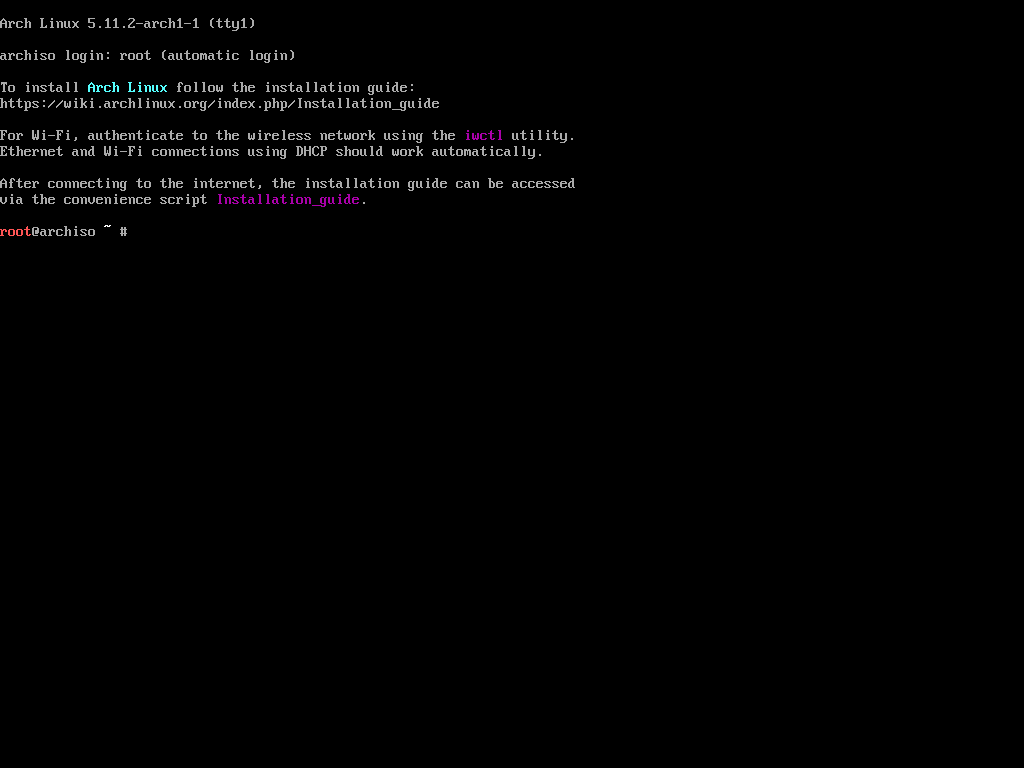
\includegraphics[width=0.7\textwidth]{images/arch1.png}
    \end{figure}
\end{frame}

%------------------------------------------------
\begin{frame}{Impostare il layout della tastiera italiana}
    Noterete che il layout della tastiera di default è quello US.\\
    Per impostare il layout della tastiera in italiano digitiamo:
    \begin{block}{}
        \$ loadkeys it
    \end{block}
\end{frame}

%------------------------------------------------
\begin{frame}{Connessione ad internet}
    
\end{frame}